% ЕМТ 2023, VII клас — точен LaTeX препис от официалните файлове в Klasirane.com.
% Условия: https://klasirane.com/api/competitions/EMT/All/2023/7%20%D0%BA%D0%BB/probs
% SHA-256 (условия): d3ce3a6e1cd6adc3372b1233e25b403c29ed8231dd74cf8086b4d71264bc8ee7
% Решения: https://klasirane.com/api/competitions/EMT/All/2023/7%20%D0%BA%D0%BB/sol
% SHA-256 (решения): b8a2e7f744f3c3a83392541683a7928390b5651cfa65eded0b16284c1531ebc0
% Точковите оценки, правописът, формулировките и видимите печатни грешки са запазени от източника.
% В повторението на условието на задача 7.2 в PDF файла с решения множителят 3b е повреден графично; условието по-долу следва официалния PDF с условията, където 3b се чете еднозначно.
% Двете схеми в решението на задача 7.4 са изрязани без редакция от растеризация на официалния PDF с решенията.

Задача 7.1. В правоъгълна координатна система $Oxy$ с единична отсечка 1 cm започват да се движат едновременно точките $A$ и $B$. Точка $A$ тръгва от $(-6;0)$ и се движи по абсцисната ос в положителна посока със скорост 2 cm/min. Точка $B$ тръгва от $(0;4)$ и се движи по ординатната ос в отрицателна посока със скорост 1 cm/min.

а) Колко сантиметра е дължината на отсечката $AB$, когато са изминали точно 9 минути след началото на движението?

б) Ако с $S$ е означено разстоянието между $A$ и $B$ точно $n$ минути след тръгването им, изразете $S^2$ чрез $n$ и представете $S^2$ като многочлен в нормален вид.

в) Колко минути след тръгването на точките $A$ и $B$ разстоянието между тях ще е минимално?

Решение. а) Девет минути след началото на движението $A$ е в точката $(12;0)$, а $B$ е в точката $(0;-5)$. От теоремата на Питагор за $\triangle OAB$ следва, че $AB^2=OA^2+OB^2=12^2+5^2=169=13^2$. Следователно $AB=13$ cm.

б) При $n=3$, $OA=0$, $OB=1$ cm, $AB=1$ и $S^2=1$.

При $n=4$, $OB=0$, $OA=2$ cm, $AB=2$ и $S^2=4$.

При $n\ne3$ и $n\ne4$, $OA=|2n-6|$ и $OB=|n-4|$. Тогава от $\triangle OAB$ според теоремата на Питагор следва, че
$$
S^2=AB^2=OA^2+OB^2=(2n-6)^2+(n-4)^2=5n^2-32n+52.
$$
Резултатът остава в сила и за частните случаи $n=3$ и $n=4$.

Отговор. $5n^2-32n+52$.

в) Тъй като
$$
S^2=5n^2-32n+52=5(n^2-2\cdot3{,}2n+10{,}24)+0{,}8=5(n-3{,}2)^2+0{,}8
$$
и $(n-3{,}2)^2\ge0$, то $S$ ще е минимално при $n=3{,}2$.Оценяване. а) 1 точка; б) 3 точки; в) 2 точки.

Задача 7.2. Даден е триъгълник $ABC$ със страни $AB=c$ cm, $BC=a$ cm, $CA=b$ cm и за които е изпълнено равенството
$$
26a^2+25b^2+25c^2+25=10a(3b+4c+1).
$$
a) Да се намери лицето на триъгълника $ABC$.

б) Построени са права $m$ през върха $A$, успоредна на $BC$, точка $P$ върху страната $AC$ така, че $AP:PC=1:2$ и пресечната точка $D$ на правите $m$ и $BP$. Намерете лицето на четириъгълника $ABCD$.

Решение. а) Преобразуваме израза до
$$
(a-5)^2+(3a-5b)^2+(4a-5c)^2=0.
$$
Тъй като $(a-5)^2\ge0$, $(3a-5b)^2\ge0$, $(4a-5c)^2\ge0$, то равенството е възможно само при $a-5=3a-5b=4a-5c=0$, откъдето намираме, че $a=5$, $b=3$, $c=4$. И тъй като $a^2=b^2+c^2$, даденият триъгълник е правоъгълен с хипотенуза $a$ и катети $b$ и $c$, откъдето следва, че лицето му $S=\dfrac{bc}{2}=\dfrac{3\cdot4}{2}=6$ cm$^2$.

б) Намираме $AP=\dfrac13\cdot AC=1$ cm, $PC=2$ cm, $S_{APB}=\dfrac{1\cdot4}{2}=2$ cm$^2$ и $S_{CPB}=6-2=4$ cm$^2$.

В трапеца $CBAD$ имаме равенството на лицата $S_{DPC}=S_{APB}=2$ cm$^2$. От
$$
\frac{S_{DPC}}{S_{DPA}}=\frac{PC}{PA}=\frac{S_{BPC}}{S_{BPA}}
$$
намираме $S_{DPA}=\dfrac{2\cdot2}{4}=1$ cm$^2$ и тогава $S_{ABCD}=6+2+1=9$ cm$^2$.

Оценяване. а) 4 точки: за представяне на израза като сбор на квадрати – 2 точки; обосновка и намиране на $a$, $b$, $c$ – 1 точка; обосновка на правоъгълния триъгълник и намиране на лицето – 1 точка; б) 2 точки.

Задача 7.3. За всяко естествено число $n$ означаваме
$$
S_n=1+2+2^2+2^3+\cdots+2^n.
$$
а) Намерете сбора на всички различни прости делители на $S_{23}$.

б) Докажете, че стойността на израза
$$
A=S_{2023}+\frac{S_{2023}+1}{2^{1012}}+2
$$
не е просто число.

в) Намерете всички естествени числа $n$, за които съществува цяло число $k$, за което
$$
S_n=1+3^k+7^k.
$$

Решение. Имаме
$$
1+2S_n=1+2(1+2+2^2+2^3+\cdots+2^n)=1+2+2^2+2^3+\cdots+2^n+2^{n+1}=S_n+2^{n+1},
$$
т.е. $1+2S_n=S_n+2^{n+1}$, откъдето следва, че $S_n=2^{n+1}-1$.

a) Разлагаме на множители:
$$
S_{23}=(2^{12})^2-1=(2^{12}-1)(2^{12}+1)=(2^4-1)(2^8+2^4+1)(2^4+1)(2^8-2^4+1)=
$$
$$
=15.273.17.241=3.5.3.7.13.17.241.
$$
Търсеният сбор е $3+5+7+13+17+241=286$.

б) Имаме
$$
A=2^{2024}-1+2^{2024}:2^{1012}+2=2^{2024}+2^{1012}+1=2^{2024}+2.2^{1012}+1-2^{1012}=
$$
$$
=(2^{1012}+1)^2-(2^{506})^2=(2^{1012}-2^{506}+1)(2^{1012}+2^{506}+1),
$$
с което е доказано, че $A$ е произведение на две естествени числа, по-големи от 1.

в) Търсим естествени числа $n$ и цели числа $k$, за които е изпълнено равенството
$$
2^{n+1}-1=1+3^k+7^k\Longleftrightarrow2^{n+1}=2+3^k+7^k.
$$
При $n=1$ равенството е изпълнено при $k=0$.

При $n\ge2$ лявата страна на равенството се дели на 8.

При нечетно $k$ имаме $3^k\equiv3\pmod8$, $7^k\equiv7\pmod8$, следователно $2+3^k+7^k\equiv4\pmod8$ и равенството е невъзможно.

При четно $k$ имаме $3^k\equiv1\pmod8$, $7^k\equiv1\pmod8$, следователно $2+3^k+7^k\equiv4\pmod8$ и отново равенството е невъзможно.

Следователно $n=1$ е единственото решение.

Оценяване. Доказателство на формулата за $S_n$ – 1 точка; а) 2 точки; б) 2 точки; в) 2 точки.

Задача 7.4. Дадени са числата
$$
1,\ 1,\ 2,\ 2,\ 3,\ 3,\ldots,\ n,\ n
$$
(всяко естествено число от 1 до $n$ е записано по два пъти). Ще казваме, че една подредба на дадените числа е хубава, ако между двете единици в получената редица има точно едно число, между двете двойки има точно две числа и т.н., за всяко $k=1,2,\ldots,n$ между двете числа $k$ в редицата има точно $k$ на брой числа.

Например, хубава подредба при $n=3$ е $3,1,2,1,3,2$, а хубава подредба при $n=4$ е $4,1,3,1,2,4,3,2$.

а) Съществува ли хубава подредба при $n=15$?

б) Докажете, че при $n=2022$ не съществува хубава подредба на числата в дадената редица.

Решение. a) Една хубава подредба при $n=15$ е:
$$
12,10,8,14,5,3,1,15,1,3,5,8,10,12,7,13,11,9,14,6,4,2,7,15,2,4,6,9,11,13.
$$

б) Да допуснем, че съществува хубава подредба. Да номерираме позициите на дадените 4044 числа отляво надясно.

Нека $a_1$ е първата позиция, в която се появява числото 1; втората такава позиция е $a_1+2$.

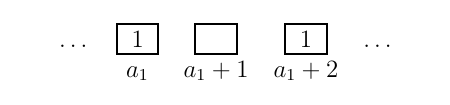
\includegraphics[max width=0.36\textwidth, alt={Позициите на двете единици в хубавата подредба}, center]{assets/7-4-positions-1.png}

Ако $a_2$ е първата позиция, в която се появява числото 2; втората такава позиция е $a_2+3$.

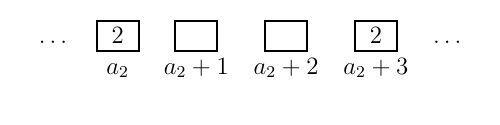
\includegraphics[max width=0.40\textwidth, alt={Позициите на двете двойки в хубавата подредба}, center]{assets/7-4-positions-2.png}

Въобще за всяко $k=1,2,\ldots,2022$ позициите, в които се появява числото $k$ в хубавата подредба означаваме с $a_k$ и $a_k+k+1$.

Сборът на всички позиции в редицата е равен на
$$
(a_1+a_2+\cdots+a_{2022})+(a_1+2+a_2+3+\cdots+a_{2022}+2023)=
$$
$$
=2(a_1+a_2+\cdots+a_{2022})+2+3+\cdots+2023=
$$
$$
=2(a_1+a_2+\cdots+a_{2022})+\frac{2023\cdot2024}{2}-1=
$$
$$
=2(a_1+a_2+\cdots+a_{2022})+2023\cdot1012-1.
$$
От друга страна, този сбор е
$$
1+2+\cdots+4044=\frac{4044\cdot4045}{2}=2022\cdot4045.
$$
Получихме, че
$$
2022\cdot4045=2(a_1+a_2+\cdots+a_{2022})+2023\cdot1012-1,
$$
което е невъзможно, тъй като лявата страна на равенството е четна, а дясната е нечетна.

Следователно при $n=2022$ не съществува хубава подредба.

Забележка. По същия начин се доказва, че не съществува хубава подредба при $n=4k+1$ и $n=4k+2$.

Оценяване: а) 3 точки; б) 4 точки.